%%===========================================================%%
%%                                                           %%
%%                   DE/DX ADJUSTMENT APPENDIX               %%
%%                                                           %%
%%===========================================================%%

\chapter{TPC track reconstruction efficiency}\label{appendix:tpcEff}


%---------------------------
\begin{figure}[hb]
\caption[TPC acceptance and reconstruction efficiency of $\pi^{-}$.]{TPC acceptance and reconstruction efficiency of $\pi^{-}$. Each plot represents the TPC efficiency $\epsilon_{\text{TPC}}$ ($z$-axis) as a function of true particle pseudorapidity $\eta$ ($x$-axis) and transverse momentum $p_{T}$ ($y$-axis) in single $z$-vertex bin whose range is given at the top. Red lines and arrows indicate region accepted in analyses.}\label{fig:tpcEff_pion_minus}
\centering
\parbox{0.495\textwidth}{
  \centering
  \includegraphics[width=\linewidth,page=3]{graphics/eff/Eff2D_TPC_pion_Minus.pdf}\\
  \includegraphics[width=\linewidth,page=5]{graphics/eff/Eff2D_TPC_pion_Minus.pdf}\\
  \includegraphics[width=\linewidth,page=7]{graphics/eff/Eff2D_TPC_pion_Minus.pdf}\\
  \includegraphics[width=\linewidth,page=9]{graphics/eff/Eff2D_TPC_pion_Minus.pdf}
}~
\parbox{0.495\textwidth}{
  \centering
  \includegraphics[width=\linewidth,page=4]{graphics/eff/Eff2D_TPC_pion_Minus.pdf}\\
  \includegraphics[width=\linewidth,page=6]{graphics/eff/Eff2D_TPC_pion_Minus.pdf}\\
  \includegraphics[width=\linewidth,page=8]{graphics/eff/Eff2D_TPC_pion_Minus.pdf}\\
  \includegraphics[width=\linewidth,page=10]{graphics/eff/Eff2D_TPC_pion_Minus.pdf}
}%
\end{figure}
\begin{figure}[hb]\ContinuedFloat
% ~\\[32pt]
\centering
\parbox{0.495\textwidth}{
  \centering
  \includegraphics[width=\linewidth,page=11]{graphics/eff/Eff2D_TPC_pion_Minus.pdf}\\
  \includegraphics[width=\linewidth,page=13]{graphics/eff/Eff2D_TPC_pion_Minus.pdf}\\
  \includegraphics[width=\linewidth,page=15]{graphics/eff/Eff2D_TPC_pion_Minus.pdf}\\
  \includegraphics[width=\linewidth,page=17]{graphics/eff/Eff2D_TPC_pion_Minus.pdf}
}~
\parbox{0.495\textwidth}{
  \centering
  \includegraphics[width=\linewidth,page=12]{graphics/eff/Eff2D_TPC_pion_Minus.pdf}\\
  \includegraphics[width=\linewidth,page=14]{graphics/eff/Eff2D_TPC_pion_Minus.pdf}\\
  \includegraphics[width=\linewidth,page=16]{graphics/eff/Eff2D_TPC_pion_Minus.pdf}\\
  \includegraphics[width=\linewidth,page=18]{graphics/eff/Eff2D_TPC_pion_Minus.pdf}
}%
\end{figure}
%---------------------------

%---------------------------
\begin{figure}[hb]
\caption[TPC acceptance and reconstruction efficiency of $\pi^{+}$.]{TPC acceptance and reconstruction efficiency of $\pi^{+}$. Each plot represents the TPC efficiency $\epsilon_{\text{TPC}}$ ($z$-axis) as a function of true particle pseudorapidity $\eta$ ($x$-axis) and transverse momentum $p_{T}$ ($y$-axis) in single $z$-vertex bin whose range is given at the top. Red lines and arrows indicate region accepted in analyses.}\label{fig:tpcEff_pion_plus}
\centering
\parbox{0.495\textwidth}{
  \centering
  \includegraphics[width=\linewidth,page=3]{graphics/eff/Eff2D_TPC_pion_Plus.pdf}\\
  \includegraphics[width=\linewidth,page=5]{graphics/eff/Eff2D_TPC_pion_Plus.pdf}\\
  \includegraphics[width=\linewidth,page=7]{graphics/eff/Eff2D_TPC_pion_Plus.pdf}\\
  \includegraphics[width=\linewidth,page=9]{graphics/eff/Eff2D_TPC_pion_Plus.pdf}
}~
\parbox{0.495\textwidth}{
  \centering
  \includegraphics[width=\linewidth,page=4]{graphics/eff/Eff2D_TPC_pion_Plus.pdf}\\
  \includegraphics[width=\linewidth,page=6]{graphics/eff/Eff2D_TPC_pion_Plus.pdf}\\
  \includegraphics[width=\linewidth,page=8]{graphics/eff/Eff2D_TPC_pion_Plus.pdf}\\
  \includegraphics[width=\linewidth,page=10]{graphics/eff/Eff2D_TPC_pion_Plus.pdf}
}%
\end{figure}
\begin{figure}[hb]\ContinuedFloat
% ~\\[32pt]
\centering
\parbox{0.495\textwidth}{
  \centering
  \includegraphics[width=\linewidth,page=11]{graphics/eff/Eff2D_TPC_pion_Plus.pdf}\\
  \includegraphics[width=\linewidth,page=13]{graphics/eff/Eff2D_TPC_pion_Plus.pdf}\\
  \includegraphics[width=\linewidth,page=15]{graphics/eff/Eff2D_TPC_pion_Plus.pdf}\\
  \includegraphics[width=\linewidth,page=17]{graphics/eff/Eff2D_TPC_pion_Plus.pdf}
}~
\parbox{0.495\textwidth}{
  \centering
  \includegraphics[width=\linewidth,page=12]{graphics/eff/Eff2D_TPC_pion_Plus.pdf}\\
  \includegraphics[width=\linewidth,page=14]{graphics/eff/Eff2D_TPC_pion_Plus.pdf}\\
  \includegraphics[width=\linewidth,page=16]{graphics/eff/Eff2D_TPC_pion_Plus.pdf}\\
  \includegraphics[width=\linewidth,page=18]{graphics/eff/Eff2D_TPC_pion_Plus.pdf}
}%
\end{figure}
%---------------------------





%---------------------------
\begin{figure}[hb]
\caption[TPC acceptance and reconstruction efficiency of $K^{-}$.]{TPC acceptance and reconstruction efficiency of $K^{-}$. Each plot represents the TPC efficiency $\epsilon_{\text{TPC}}$ ($z$-axis) as a function of true particle pseudorapidity $\eta$ ($x$-axis) and transverse momentum $p_{T}$ ($y$-axis) in single $z$-vertex bin whose range is given at the top. Red lines and arrows indicate region accepted in analyses.}\label{fig:tpcEff_kaon_minus}
\centering
\parbox{0.495\textwidth}{
  \centering
  \includegraphics[width=\linewidth,page=3]{graphics/eff/Eff2D_TPC_kaon_Minus.pdf}\\
  \includegraphics[width=\linewidth,page=5]{graphics/eff/Eff2D_TPC_kaon_Minus.pdf}\\
  \includegraphics[width=\linewidth,page=7]{graphics/eff/Eff2D_TPC_kaon_Minus.pdf}\\
  \includegraphics[width=\linewidth,page=9]{graphics/eff/Eff2D_TPC_kaon_Minus.pdf}
}~
\parbox{0.495\textwidth}{
  \centering
  \includegraphics[width=\linewidth,page=4]{graphics/eff/Eff2D_TPC_kaon_Minus.pdf}\\
  \includegraphics[width=\linewidth,page=6]{graphics/eff/Eff2D_TPC_kaon_Minus.pdf}\\
  \includegraphics[width=\linewidth,page=8]{graphics/eff/Eff2D_TPC_kaon_Minus.pdf}\\
  \includegraphics[width=\linewidth,page=10]{graphics/eff/Eff2D_TPC_kaon_Minus.pdf}
}%
\end{figure}
\begin{figure}[hb]\ContinuedFloat
% ~\\[32pt]
\centering
\parbox{0.495\textwidth}{
  \centering
  \includegraphics[width=\linewidth,page=11]{graphics/eff/Eff2D_TPC_kaon_Minus.pdf}\\
  \includegraphics[width=\linewidth,page=13]{graphics/eff/Eff2D_TPC_kaon_Minus.pdf}\\
  \includegraphics[width=\linewidth,page=15]{graphics/eff/Eff2D_TPC_kaon_Minus.pdf}\\
  \includegraphics[width=\linewidth,page=17]{graphics/eff/Eff2D_TPC_kaon_Minus.pdf}
}~
\parbox{0.495\textwidth}{
  \centering
  \includegraphics[width=\linewidth,page=12]{graphics/eff/Eff2D_TPC_kaon_Minus.pdf}\\
  \includegraphics[width=\linewidth,page=14]{graphics/eff/Eff2D_TPC_kaon_Minus.pdf}\\
  \includegraphics[width=\linewidth,page=16]{graphics/eff/Eff2D_TPC_kaon_Minus.pdf}\\
  \includegraphics[width=\linewidth,page=18]{graphics/eff/Eff2D_TPC_kaon_Minus.pdf}
}%
\end{figure}
%---------------------------


%---------------------------
\begin{figure}[hb]
\caption[TPC acceptance and reconstruction efficiency of $K^{+}$.]{TPC acceptance and reconstruction efficiency of $K^{+}$. Each plot represents the TPC efficiency $\epsilon_{\text{TPC}}$ ($z$-axis) as a function of true particle pseudorapidity $\eta$ ($x$-axis) and transverse momentum $p_{T}$ ($y$-axis) in single $z$-vertex bin whose range is given at the top. Red lines and arrows indicate region accepted in analyses.}\label{fig:tpcEff_kaon_plus}
\centering
\parbox{0.495\textwidth}{
  \centering
  \includegraphics[width=\linewidth,page=3]{graphics/eff/Eff2D_TPC_kaon_Plus.pdf}\\
  \includegraphics[width=\linewidth,page=5]{graphics/eff/Eff2D_TPC_kaon_Plus.pdf}\\
  \includegraphics[width=\linewidth,page=7]{graphics/eff/Eff2D_TPC_kaon_Plus.pdf}\\
  \includegraphics[width=\linewidth,page=9]{graphics/eff/Eff2D_TPC_kaon_Plus.pdf}
}~
\parbox{0.495\textwidth}{
  \centering
  \includegraphics[width=\linewidth,page=4]{graphics/eff/Eff2D_TPC_kaon_Plus.pdf}\\
  \includegraphics[width=\linewidth,page=6]{graphics/eff/Eff2D_TPC_kaon_Plus.pdf}\\
  \includegraphics[width=\linewidth,page=8]{graphics/eff/Eff2D_TPC_kaon_Plus.pdf}\\
  \includegraphics[width=\linewidth,page=10]{graphics/eff/Eff2D_TPC_kaon_Plus.pdf}
}%
\end{figure}
\begin{figure}[hb]\ContinuedFloat
% ~\\[32pt]
\centering
\parbox{0.495\textwidth}{
  \centering
  \includegraphics[width=\linewidth,page=11]{graphics/eff/Eff2D_TPC_kaon_Plus.pdf}\\
  \includegraphics[width=\linewidth,page=13]{graphics/eff/Eff2D_TPC_kaon_Plus.pdf}\\
  \includegraphics[width=\linewidth,page=15]{graphics/eff/Eff2D_TPC_kaon_Plus.pdf}\\
  \includegraphics[width=\linewidth,page=17]{graphics/eff/Eff2D_TPC_kaon_Plus.pdf}
}~
\parbox{0.495\textwidth}{
  \centering
  \includegraphics[width=\linewidth,page=12]{graphics/eff/Eff2D_TPC_kaon_Plus.pdf}\\
  \includegraphics[width=\linewidth,page=14]{graphics/eff/Eff2D_TPC_kaon_Plus.pdf}\\
  \includegraphics[width=\linewidth,page=16]{graphics/eff/Eff2D_TPC_kaon_Plus.pdf}\\
  \includegraphics[width=\linewidth,page=18]{graphics/eff/Eff2D_TPC_kaon_Plus.pdf}
}%
\end{figure}
%---------------------------













%---------------------------
\begin{figure}[hb]
\caption[TPC acceptance and reconstruction efficiency of $\bar{p}$.]{TPC acceptance and reconstruction efficiency of $\bar{p}$. Each plot represents the TPC efficiency $\epsilon_{\text{TPC}}$ ($z$-axis) as a function of true particle pseudorapidity $\eta$ ($x$-axis) and transverse momentum $p_{T}$ ($y$-axis) in single $z$-vertex bin whose range is given at the top. Red lines and arrows indicate region accepted in analyses.}\label{fig:tpcEff_proton_minus}
\centering
\parbox{0.495\textwidth}{
  \centering
  \includegraphics[width=\linewidth,page=3]{graphics/eff/Eff2D_TPC_proton_Minus.pdf}\\
  \includegraphics[width=\linewidth,page=5]{graphics/eff/Eff2D_TPC_proton_Minus.pdf}\\
  \includegraphics[width=\linewidth,page=7]{graphics/eff/Eff2D_TPC_proton_Minus.pdf}\\
  \includegraphics[width=\linewidth,page=9]{graphics/eff/Eff2D_TPC_proton_Minus.pdf}
}~
\parbox{0.495\textwidth}{
  \centering
  \includegraphics[width=\linewidth,page=4]{graphics/eff/Eff2D_TPC_proton_Minus.pdf}\\
  \includegraphics[width=\linewidth,page=6]{graphics/eff/Eff2D_TPC_proton_Minus.pdf}\\
  \includegraphics[width=\linewidth,page=8]{graphics/eff/Eff2D_TPC_proton_Minus.pdf}\\
  \includegraphics[width=\linewidth,page=10]{graphics/eff/Eff2D_TPC_proton_Minus.pdf}
}%
\end{figure}
\begin{figure}[hb]\ContinuedFloat
% ~\\[32pt]
\centering
\parbox{0.495\textwidth}{
  \centering
  \includegraphics[width=\linewidth,page=11]{graphics/eff/Eff2D_TPC_proton_Minus.pdf}\\
  \includegraphics[width=\linewidth,page=13]{graphics/eff/Eff2D_TPC_proton_Minus.pdf}\\
  \includegraphics[width=\linewidth,page=15]{graphics/eff/Eff2D_TPC_proton_Minus.pdf}\\
  \includegraphics[width=\linewidth,page=17]{graphics/eff/Eff2D_TPC_proton_Minus.pdf}
}~
\parbox{0.495\textwidth}{
  \centering
  \includegraphics[width=\linewidth,page=12]{graphics/eff/Eff2D_TPC_proton_Minus.pdf}\\
  \includegraphics[width=\linewidth,page=14]{graphics/eff/Eff2D_TPC_proton_Minus.pdf}\\
  \includegraphics[width=\linewidth,page=16]{graphics/eff/Eff2D_TPC_proton_Minus.pdf}\\
  \includegraphics[width=\linewidth,page=18]{graphics/eff/Eff2D_TPC_proton_Minus.pdf}
}%
\end{figure}
%---------------------------


%---------------------------
\begin{figure}[hb]
\caption[TPC acceptance and reconstruction efficiency of $p$.]{TPC acceptance and reconstruction efficiency of $p$. Each plot represents the TPC efficiency $\epsilon_{\text{TPC}}$ ($z$-axis) as a function of true particle pseudorapidity $\eta$ ($x$-axis) and transverse momentum $p_{T}$ ($y$-axis) in single $z$-vertex bin whose range is given at the top. Red lines and arrows indicate region accepted in analyses.}\label{fig:tpcEff_proton_plus}
\centering
\parbox{0.495\textwidth}{
  \centering
  \includegraphics[width=\linewidth,page=3]{graphics/eff/Eff2D_TPC_proton_Plus.pdf}\\
  \includegraphics[width=\linewidth,page=5]{graphics/eff/Eff2D_TPC_proton_Plus.pdf}\\
  \includegraphics[width=\linewidth,page=7]{graphics/eff/Eff2D_TPC_proton_Plus.pdf}\\
  \includegraphics[width=\linewidth,page=9]{graphics/eff/Eff2D_TPC_proton_Plus.pdf}
}~
\parbox{0.495\textwidth}{
  \centering
  \includegraphics[width=\linewidth,page=4]{graphics/eff/Eff2D_TPC_proton_Plus.pdf}\\
  \includegraphics[width=\linewidth,page=6]{graphics/eff/Eff2D_TPC_proton_Plus.pdf}\\
  \includegraphics[width=\linewidth,page=8]{graphics/eff/Eff2D_TPC_proton_Plus.pdf}\\
  \includegraphics[width=\linewidth,page=10]{graphics/eff/Eff2D_TPC_proton_Plus.pdf}
}%
\end{figure}
\begin{figure}[hb]\ContinuedFloat
% ~\\[32pt]
\centering
\parbox{0.495\textwidth}{
  \centering
  \includegraphics[width=\linewidth,page=11]{graphics/eff/Eff2D_TPC_proton_Plus.pdf}\\
  \includegraphics[width=\linewidth,page=13]{graphics/eff/Eff2D_TPC_proton_Plus.pdf}\\
  \includegraphics[width=\linewidth,page=15]{graphics/eff/Eff2D_TPC_proton_Plus.pdf}\\
  \includegraphics[width=\linewidth,page=17]{graphics/eff/Eff2D_TPC_proton_Plus.pdf}
}~
\parbox{0.495\textwidth}{
  \centering
  \includegraphics[width=\linewidth,page=12]{graphics/eff/Eff2D_TPC_proton_Plus.pdf}\\
  \includegraphics[width=\linewidth,page=14]{graphics/eff/Eff2D_TPC_proton_Plus.pdf}\\
  \includegraphics[width=\linewidth,page=16]{graphics/eff/Eff2D_TPC_proton_Plus.pdf}\\
  \includegraphics[width=\linewidth,page=18]{graphics/eff/Eff2D_TPC_proton_Plus.pdf}
}%
\end{figure}
%---------------------------